\section{Multitask pretraining}

\newcommand{\featureplot}[2]{
    \begin{tikzpicture}
        \begin{axis}[
            view={0}{90},
            colorbar,
            colormap/temp,
            mesh/cols=64,
            height=7cm,
            width=7cm,
            xmajorticks=false,
            ymajorticks=false,
            xlabel={Features},
            ylabel={Features},
            point meta min=#2,
            point meta max=1,
            xmin=-0.5,
            xmax=63.5,
            ymin=-0.5,
            ymax=63.5,
            colorbar style={
                tick style={draw=none}
            }
        ]
        \addplot [
            matrix plot,
            mesh/cols=64,
            point meta=explicit,
            draw=black,
            draw opacity=0.1
        ] table [col sep=comma, meta index=2] {#1};

        \end{axis}
    \end{tikzpicture}
}

\newsavebox{\featurecorrelations}
\sbox{\featurecorrelations}{
    \featureplot{data/feature_correlations.csv}{0}
}
\newsavebox{\multicorrelations}
\sbox{\multicorrelations}{
    \featureplot{data/sfcn-multi.csv}{-1}
}

\newcommand{\bapredictions}[4]{
    \ifnum#4=1
        \def\annotations{, xlabel={Chronological age}, ylabel={Predicted age}}%
    \else
        \def\annotations{, yticklabels={,,}}%
    \fi
    \begin{tikzpicture}
        \begin{axis}[
            height=5.7cm,
            width=5.7cm,
            xmin=0,
            xmax=100,
            ymin=0,
            ymax=100,
            xtick pos=bottom,
            ytick pos=left,
            title=#2,
            xtick style={draw=none},
            ytick style={draw=none},
            xmajorgrids=true,
            ymajorgrids=true,
            clip=false,
            title style={text depth=0, font=\large\bfseries},
            \annotations
        ]
            \addplot[thick] coordinates {(0, 0) (100, 100)};
            \addplot[
                only marks,
                mark=*,
                blue,
                opacity=0.1,
                mark options={
                    scale=0.5
                }
            ] table [
                col sep=comma,
                x=true,
                y=predicted
            ] {#1};
            \node[anchor=south east, font=\small\bfseries, text=red] at (rel axis cs: 1, 0) {
                MAE=#3
            };
        \end{axis}
    \end{tikzpicture}
}

\newsavebox{\bareg}
\sbox{\bareg}{
    \bapredictions{data/reg_test_age.csv}{Brain age}{3.68}{1}
}
\newsavebox{\bamulti}
\sbox{\bamulti}{
    \bapredictions{data/multi_test_age.csv}{Multitask}{3.41}{0}
}

\newcommand{\tltrace}[3]{
    \addplot[
        #2,
        mark=*,
        draw opacity=0.75,
        fill opacity=0.75,
        thick,
        mark options={
            scale=1.5
        }
    ] table [
        col sep=comma,
        x=size,
        y=#2_#3_mean
    ] {#1};
}


\newsavebox{\tlbrainage}
\sbox{\tlbrainage}{
    \begin{tikzpicture}
        \begin{axis}[
            height=7cm,
            width=10cm,
            xtick pos=bottom,
            ytick style={draw=none},
            ymajorgrids=true,
            xlabel={Dataset size},
            ylabel=Out-of-sample\\relative absolute error,
            title=\textbf{Retraining a brain age model},
            legend style={
                font=\footnotesize
            },
            legend cell align={left},
            ylabel style={align=center},
            title style={yshift=-0.15cm, text depth=0}
        ]
            \tltrace{data/age_top.csv}{none}{loss}
            \tltrace{data/age_top.csv}{pretrained}{loss}
            \tltrace{data/age_top.csv}{freeze}{loss}
            \tltrace{data/age_top.csv}{finetune}{loss}

            \addlegendentry{Baseline}
            \addlegendentry{Pretrained (frozen)}
            \addlegendentry{Pretrained (extraction)}
            \addlegendentry{Pretrained (finetuned)}
        \end{axis}
    \end{tikzpicture}
}

\newsavebox{\tlad}
\sbox{\tlad}{
    \begin{tikzpicture}
        \begin{axis}[
            height=7cm,
            width=10cm,
            xtick pos=bottom,
            ytick style={draw=none},
            ymajorgrids=true,
            xlabel={Dataset size},
            ylabel=Out-of-sample\\area under the ROC curve,
            title=\textbf{Retraining an AD classifier},
            legend style={
                font=\footnotesize,
                anchor=south east,
                at={(0.95, 0.05)}
            },
            legend cell align={left},
            ylabel style={align=center},
            title style={yshift=-0.15cm, text depth=0}
        ]
            \tltrace{data/ad.csv}{none}{loss}
            \tltrace{data/ad.csv}{freeze}{loss}
            \tltrace{data/ad.csv}{finetune}{loss}

            \addlegendentry{Baseline}
            \addlegendentry{Pretrained (extraction)}
            \addlegendentry{Pretrained (finetuned)}
        \end{axis}
    \end{tikzpicture}
}

\begin{frame}{Multitask pretraining}
    \begin{tikzpicture}
        \node[] at (-5.25, -3.75) {};
        \node[] at (5.25, 3.5) {};

        \def\xmin{-2.55}
        \def\ymin{1}
        \def\nodedepth{0.066}
        \def\nodesize{0.15}

        \visible<1>{
            \node[anchor=south, text depth=0] at (\xmin + 2.675, \ymin + 1.43) {
                \textbf{Convolutional neural network}
            };
            \draw[thick, dashed] (\xmin + 0.22, \ymin + 1.43) --
            (\xmin + 5.13, \ymin + 1.43) --
            (\xmin + 5.13, \ymin - 1.42) --
            (\xmin + 0.22, \ymin - 1.42) -- cycle;

            \convlayer{\xmin - 0.06 + 0.4}{\ymin + 2.5 * \nodesize}{\nodedepth}{\nodesize}{12}{3}{blue}

            \node[] (firstfeatures) at (-0.95, -2) {
                \usebox{\firstfeaturespace}
            };

            \cnnarrow{(\xmin + 0.95, \ymin)}{(\xmin+2.2, \ymin)}{blue}
            \convlayer{\xmin + 1.44 + 0.4}{\ymin + 1.5 * \nodesize}{\nodedepth}{\nodesize}{8}{5}{blue}

            \node[] (secondfeatures) at (0.38, -2) {
                \usebox{\secondfeaturespace}
            };

            \cnnarrow{(\xmin + 2.43, \ymin)}{(\xmin+3.5, \ymin)}{blue}
            \convlayer{\xmin + 2.77 + 0.4}{\ymin + 0.5 * \nodesize}{\nodedepth}{\nodesize}{4}{7}{blue}

            \node[] (thirdfeatures) at (1.56, -2) {
                \usebox{\thirdfeaturespace}
            };

            \cnnarrow{(\xmin + 3.75, \ymin)}{(\xmin+5, \ymin)}{blue}
            \convlayer{\xmin + 3.93 + 0.4}{\ymin + 0}{\nodedepth}{\nodesize}{2}{9}{blue}

        }
        \visible<2-3>{
            \node[inner sep=0pt, draw=black] at (0, 2) {
                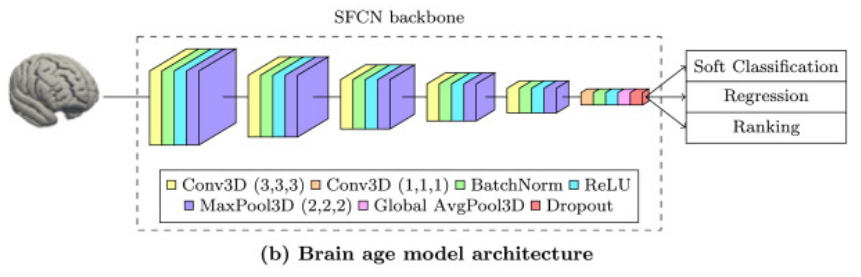
\includegraphics[width=8cm]{data/brainagemodel.png}
            };

            \node[anchor=south, text width=10.5cm, font=\tiny, align=flush center] at (0, -3.95) {
                Leonardsen, E. H., Peng, H., Kaufmann, T., Agartz, I., Andreassen, O. A., Celius, E. G., ... \& Wang, Y. (2022). "Deep neural networks learn general and clinically relevant representations of the ageing brain". \textit{NeuroImage, 256}, 119210.
            };
        }
        \visible<3>{
            \node[text width=10.5cm, align=flush center] at (0, -1.4) {
                \textit{"Furthermore, we see this result as evidence that deep learning models trained to predict age in large multisite datasets constitute excellent starting points for transfer learning, which can subsequently be fine-tuned to a variety of tasks."}\\
                - Esten et al.
            };
        }
        \visible<4>{
            \node[inner sep=0pt, draw=black] at (0, 0) {
                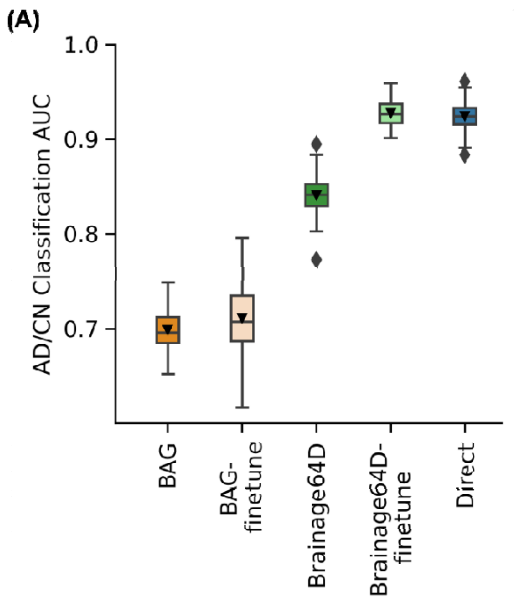
\includegraphics[width=4.5cm]{data/yeo.png}
            };
            \node[anchor=south, text width=10.5cm, font=\tiny, align=flush center] at (0, -3.95) {
                Tan, T. W. K., Nguyen, K. N., Zhang, C., Kong, R., Cheng, S. F., Ji, F., ... \& B. T. Thomas Yeo. (2024). "Evaluation of Brain Age as a Specific Marker of Brain Health". \textit{bioRxiv}, 2024-11.
            };
        }
        \visible<5>{
            \node[] at (0, 0) {
                \usebox{\multitaskbrainage}
            };
            \node[draw=red, thick, minimum height=1.2cm, minimum width=0.1cm] at (0.99, 0) {};
        }
        \visible<6>{
            \node[] at (0, 0) {
                \usebox{\featurecorrelations}
            };
        }
        \visible<7>{
            \node[] at (0, 0) {
                \usebox{\multitaskmultitask}
            };
        }
        \visible<8>{
            \node[] at (0, 0) {
                \usebox{\multicorrelations}
            };
        }
        \visible<9>{
            \node[] at (-2.4, 0) {
                \usebox{\bareg}
            };
            \node[] at (2.8, 0.29) {
                \usebox{\bamulti}
            };
        }
        \visible<10>{
            \node[] at (0, 0) {
                \usebox{\tlbrainage}
            };
        }
        \visible<11>{
            \node[] at (0, 0) {
                \usebox{\tlad}
            };
        }
    \end{tikzpicture}
\end{frame}
